\documentclass[a4paper,12pt]{article}

\usepackage[utf8]{inputenc}
\usepackage[catalan]{babel}
\usepackage{amssymb}
\usepackage{amsmath}
\usepackage{amsthm}
\usepackage[pdftex]{graphicx}
\usepackage[pdftex]{color}
\usepackage[colorlinks,linkcolor=black,citecolor=black,urlcolor=black]{hyperref}
\usepackage[all]{xy}

\newtheorem{teo}{Teorema}
\newtheorem{pro}{Proposició}

\title{El meu treball a \LaTeX}
\author{Pol Piñol Castuera}
\date{}

\begin{document}
\maketitle
\tableofcontents
\section{Introducció}
L'objectiu d'aquest treball és avaluar el coneixement de l'editor de text \LaTeX.
A la Secció \ref{sec:alg} hi utilitzem un tema d'Algebra Lineal i a la Secció \ref{sec:clc} un de Càlcul Diferencial. % hyperlink 2 i 3
\section{Àlgebra lineal}\label{sec:alg}
En aquesta secció recordem algunes propietats de la matriu associada a una
aplicació lineal. En cap moment pretenem ser exhaustius. Per a aprofundir
en el tema referim el lector a l'assignatura \textit{Àlgebra lineal} del primer curs
de Grau de Matemàtiques i a la bibliografia d'aquesta assignatura com ara
per exemple \cite{1}, \cite{2}. La pàgina web interactiva \cite{3} és un recurs més bàsic on s'expliquen pas a pas les nocions d'Àlgebra Lineal amb molts exemples i il·lustracions.
\subsection{Aplicacions lineals}
En tota la secció suposem que
\begin{itemize}
\item \textit{V},\textit{W} són espais vectorials sobre $\mathbb{R}$
\item $\mathcal{B} = \{v_{1},\ldots, v_{n} \}$ és una base ordenada de \textit{V}.
\item $\overline{\mathcal{B}}=\{w_{1},\ldots, w_{n} \}$ és una base ordenada de \textit{W}.
\item \textit{T} : \textit{V} $\rightarrow$ \textit{W} és una aplicació lineal entre els espais vectorials \textit{V} i \textit{W}.
\end{itemize}

\paragraph{Coordenades d'un vector.}  Per cada vector $v \in V$ existeixen $x_{1}, \ldots, x_{n} \in \mathbb{R}$ únics de manera que $v =\sum_{i=1}^n x_{i}v_{i}$. El vector $(x_{1}, \ldots, x_{n})$ s'anomena vector de les coordenades de \textit{v} respecte de la base $\mathcal{B}$, i el denotem per \begin{equation} [v]_{\mathcal{B}}=(x_{1}, \ldots, x_{n}).  \end{equation}


\paragraph{Matriu associada a una aplicació lineal.} La matriu associada a \textit{T} respecte de les bases $\mathcal{B}$ en $\overline{\mathcal{B}}$ està donada per \begin{equation}
m(T)_{\mathcal{B},\overline{\mathcal{B}}} = \left( \  \begin{tabular}{|c|c|c|c|}
\hline & & & \\ $[T(v_{1})]_{\overline{\mathcal{B}}}$ & $[T(v_{2})]_{\overline{\mathcal{B}}}$ & \ldots \ldots & $[T(v_{n})]_{\overline{\mathcal{B}}}$ \\ & & & \\
 \hline
 \end{tabular} \ \right), \end{equation} on la \textit{i}-èsima columna està formada per les coordenades de $T(v_{i})$ respecte de la base $\overline{\mathcal{B}}$. Notem que, per cada $v \in V$, les coordenades de $T(v)$ respecte de $\overline{\mathcal{B}}$ estan donades per \begin{equation} \label{eq:3} [T(v)]_{\overline{\mathcal{B}}}= m(T)_{\mathcal{B},\overline{\mathcal{B}}} \cdot [v]_{\mathcal{B}}, \end{equation} on els vectors de coordenades $[v]_{\mathcal{B}}$ i $[T(v)]_{\overline{\mathcal{B}}}$ estan considerats com matrius de dimensió $n \times 1$ i $m \times 1$ respectivament. Aleshores, si $[T(v)]_{\overline{\mathcal{B}}}=(y_{1},\ldots,y_{m})$, llavors $T(v)=\sum_{i=1}^m y_{i}w_{i}$.
\paragraph{Matriu de l'aplicació lineal inversa.} Si \textit{T} : \textit{V} $\rightarrow$ \textit{W} és un isomorfisme, aleshores dim\textit{V}=dim\textit{W}, $m(T)_{\mathcal{B},\overline{\mathcal{B}}}$ és invertible i la seva matriu és: $$(m(T)_{\mathcal{B},\overline{\mathcal{B}}})^{-1}= m(T^{-1})_{\overline{\mathcal{B}},\mathcal{B}}.$$
Esquemàticament,

\begin{equation}
\xymatrix{ [v]_{\mathcal{B}} \ar@/^2pc/[rr]^{m(T)_{\mathcal{B},\overline{\mathcal{B}}}}  &   & [T(v)]_{\overline{\mathcal{B}}} \ar@/^2pc/[ll]^{m(T^{-1})_{\overline{\mathcal{B}},\mathcal{B}}}}
\end{equation}
on tenim a l'esquerra les coordenades del vector \textit{v} respecte de la base $\mathcal{B}$ i a la dreta les coordenades del vector $T(v)$ respecte de la base $\overline{\mathcal{B}}$.

\paragraph{Teorema fonamental de les transformacions lineals} El teorema següent dóna condicions suficients i necessàries perquè existeixi una aplicació lineal única que transforma una figura geomètrica donada en una altra. Després, com a il·lustració, treballarem un exemple en l'espai vectorial $\mathbb{R}^{2}$. \begin{teo}
Siguin V,W espais vectorials, sigui $\mathcal{B}=\{v_{1},v_{2},\ldots,v_{n}\}$ una base de V i siguin $w_{1},w_{2},\ldots,w_{n}$ vectors arbitraris (iguals o no) de W. Aleshores existeix una única aplicació lineal $T : V \rightarrow W$ que compleix $T(v_{i}) = w_{i}, \ 1 \leq i \leq n$. \label{teo:1}
\end{teo}


La demostració d'aquest teorema es pot trobar a \cite{1}. Tot seguit expliquem com trobar l'aplicació lineal T en un cas concret.

Anem a veure si podem transformar el triangle que hi ha a l'esquerra en el triangle que hi ha a la dreta (\ref{eq:(5)}):
\begin{equation}
\xymatrix{ 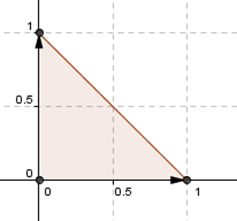
\includegraphics[width=3cm]{Teoremafund1.png} \ar@/_2pc/[rr]^{T}  &   & 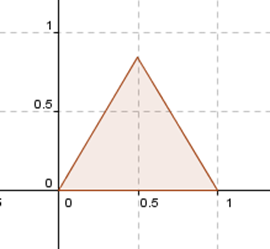
\includegraphics[width=3.5cm]{Teoremafund2.png}} \label{eq:(5)}
\end{equation}
Pel Teorema \ref{teo:1}, una aplicació lineal únicament per les imatges d'una base de $\mathbb{R}^2$. Observem que la base canònica, $\mathcal{B}={(1,0),(0,1)}$, determina el primer triangle. D'acord amb això, li assignem les següents imatges transformades per \textit{T}:
$$\begin{cases}
T ((1,0)) =(1,0),\\
T ((0,1)) =(\frac{1}{2},1).
\end{cases}$$
Per trobar la fórmula analítica de l'aplicació lineal \textit{T} podem utilitzar (\ref{eq:3}) tot observant que les coordenades són els vectors mateixos si triem com a bases ordenades $\mathcal{B}=\overline{\mathcal{B}}$ la base canònica de $V=W=\mathbb{R}^2$. Sigui $v=(x,y)$ un vector genèric de $\mathbb{R}^2$, aleshores la seva imatge transformada per \textit{T} és:
$$T\big( (x,y) \big)=m(T)_{\mathcal{B},\mathcal{B}} \cdot \binom{x}{y}=\binom{x+\frac{1}{2}y}{y}=(x+\dfrac{1}{2}y,y) .$$

\section{Càlcul Diferencial}\label{sec:clc}
Recordem aquí una propietat de la derivada de funcions d'una variable.

\begin{pro}
Suposem $r > 1$ és una constant i $f : I \subset \mathbb{R} \rightarrow \mathbb{R}$ és una funció que compleix la desigualtat $f(x) \le |x|^{r}$ per cada x en I, on I és un interval obert que conté 0. Aleshores f és diferenciable en $x=0$.
\end{pro}

\begin{proof}
La desigualtat $f(x) \leq |x|^{r}$ amb $r>1$ implica que $f(0)=0$. Per tant tenim que
$$\left|\frac{f(x)-f(0)}{x-0}\right|=\left|\frac{f(x)}{x}\right| \leq |x|^{r-1}.$$
Com que $r-1 >0$, tenim $\lim\limits_{x \to 0}|x|^{r-1}=0$, per la qual cosa obtenim que
\begin{align}
\lim\limits_{x \to 0}\left|\frac{f(x)-f(0)}{x-0}\right|=0 \ \nonumber \\
\Leftrightarrow\lim\limits_{x \to 0}\frac{f(x)-f(0)}{x-0}=0. \label{eq:6}
\end{align}
Llavors, d'acord amb la definició de diferenciabilitat, (\ref{eq:6}) diu que \textit{f} és diferenciable en $x=0$ amb derivada $f'(0)=0$.
\end{proof}

\begin{thebibliography}{3}

\bibitem{1}
F. Cedo, A. Reventós. \textit{Geometria plana i Algebra lineal.} Manuals de la UAB, Servei de Publicacions, UAB, Bellaterra, 2004.

\bibitem{2}
L. Merino i E. Santos. \textit{Àlgebra lineal con métodos elementales.} Ed. Thomson, Madrid, 2006.

\bibitem{3}
F. Gómez, I. Pustilnik. \textit{Álgebra y Geometría Analítica Online!} \url{https://aga.frba.utn.edu.ar}, 2017.



\end{thebibliography}


\end{document}

